% SPDX-License-Identifier: CC-BY-4.0
% Copyright (C) 2026 Fabian Januszewski, Abhijit (the Langlandscape team)
\section{The hypotheses report}\label{app:hyp}
The following pages reproduce, unchanged, the hypotheses report \cite{LLhyp}
(\texttt{mathematics/report/standalone-hypotheses.pdf}, 21 pp.) as of its date (15 November 2026; its registry snapshot and
the gate table it quotes are those named on its title page, and it calls itself provisional). It has since been partly
superseded: FD1 and FD2 are decided and stage 06 is closed (its \texttt{RamNrdSurj} entry already records the discharge). The final state is the one given in the main text,
\S\ref{sec:lean} (from the milestone closure S06 and \texttt{HYPOTHESES.md} at c70ef3a9: \GateAudited/\GateAudited{} audited declarations at the final gate bsf-gate-1,
\NumHypRegistered{} registered hypotheses). In its Table~1, ``discharged'' for \texttt{ResidualBurnside} means discharged given absolute irreducibility, (H2). Page numbers and cross-references on the following pages are those of the report itself.
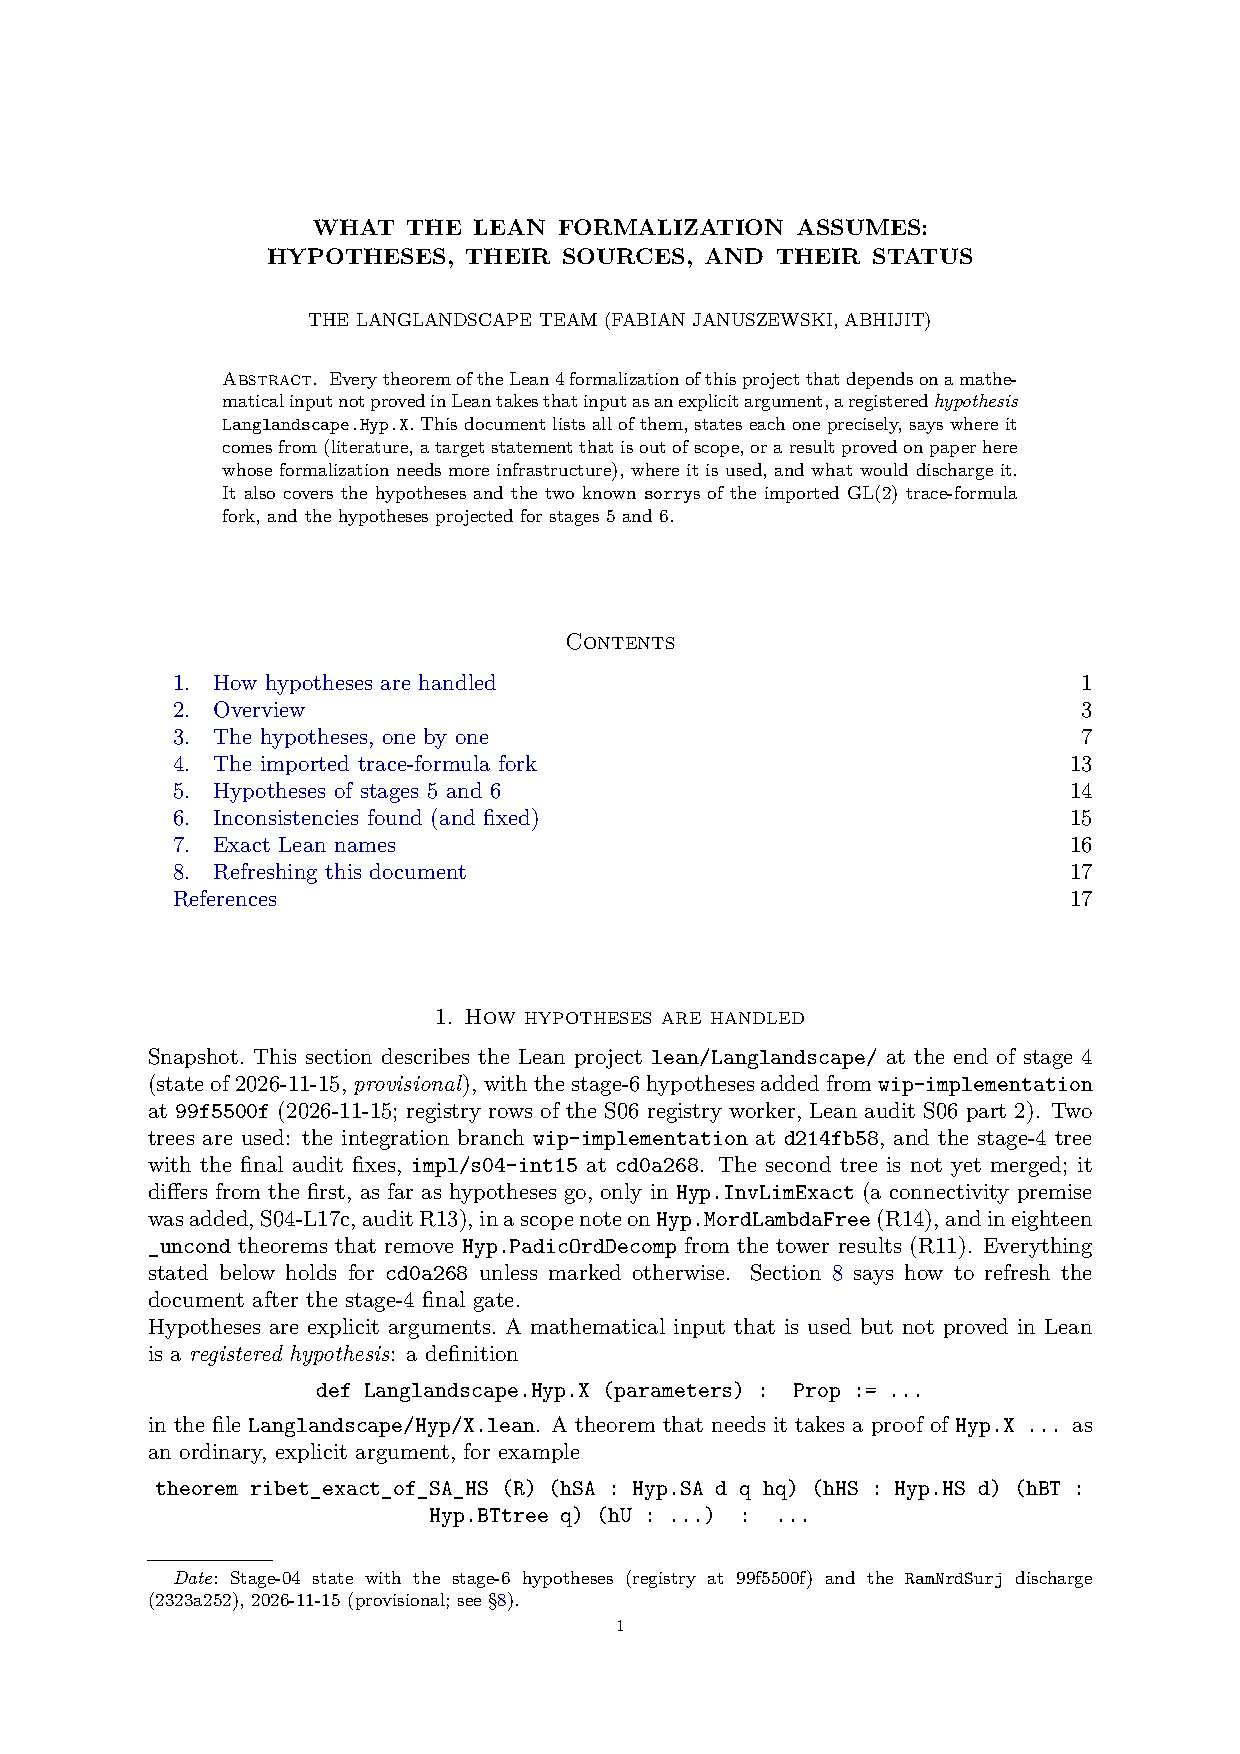
\includepdf[pages=-,scale=0.9,frame,pagecommand={\thispagestyle{plain}}]{../report/standalone-hypotheses.pdf}
